\documentclass{article}
\usepackage{listings}
\usepackage{graphicx}
\usepackage{float}
\usepackage{fontspec}
\setmainfont{Ubuntu}
\setsansfont{Ubuntu}% Ubuntu as sans - use \sffamily or \textsf{} as normal
\setmonofont{JetBrainsMono Nerd Font Mono}% Ubuntu Mono as 'typewriter' - use \ttfamily or \texttt{}
\usepackage[a4paper,
            bindingoffset=0.2in,
            left=1cm,
            right=1cm,
            top=1in,
            bottom=1in,
            footskip=.25in]{geometry}
\usepackage{hyperref}
\hypersetup{
    colorlinks, citecolor=black, filecolor=black,
    linkcolor=black, urlcolor=black
}
\usepackage{xcolor}
\definecolor{mygreen}{rgb}{0.05,0.15,0.11}
\definecolor{mygray}{rgb}{0.9,0.9,0.9}
\definecolor{mymauve}{rgb}{0.58,0,0.82}
\lstset{
  % backgroundcolor=\color{mygray}, 
  basicstyle=\ttfamily,
  breakatwhitespace=false,
  breaklines=true,
  % commentstyle=\color{darkgray},
  keepspaces=true,
  keywordstyle=\bfseries,
  morekeywords={*,...},
  showspaces=false,
  showstringspaces=false,
  showtabs=false,
  % stringstyle=\color{blue},
  tabsize=4,
  % numbers=left,
  rulecolor=\color{black},
  postbreak=\mbox{\textcolor{red}{$\hookrightarrow$}\space}
}

\begin{document}

\pagenumbering{gobble}

{\centerline{\bfseries \Huge Assignment 9}}

\section*{Question 1}
Write PHP code to demonstrate sorting in associative arrays and
also use some numeric keys.
\subsection*{Code}
\lstinputlisting[language=php]{1/index.php}
\subsection*{Output}
\begin{figure}[H]
  \centering
  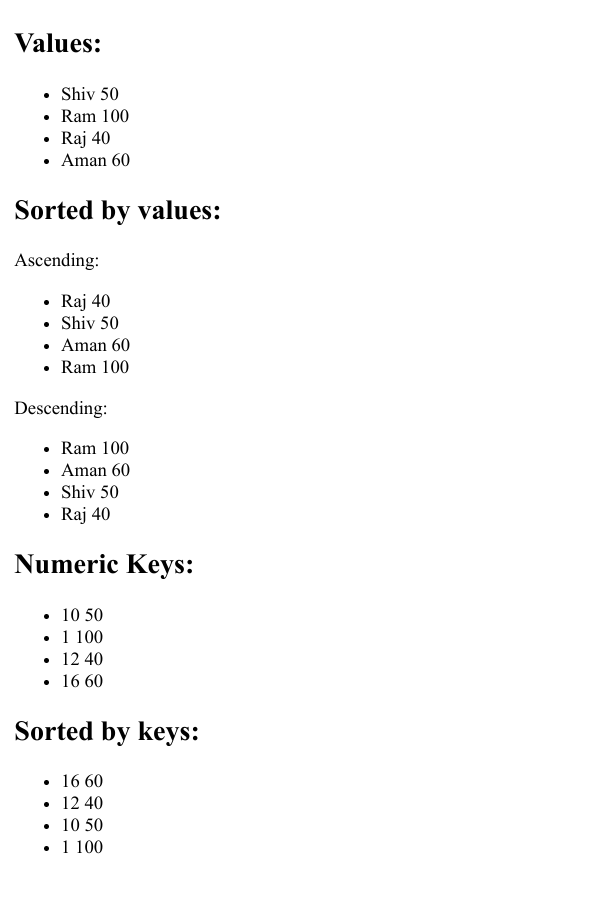
\includegraphics[width=10cm]{1/out.png}
\end{figure}

\newpage
\section*{Question 2}
Write PHP code read character by character from a file and write all
the vowels into another file.
\subsection*{Code}
\lstinputlisting[language=php]{2/index.php}
\subsection*{Output}
\textbf{input.txt}
\lstinputlisting[language=php]{2/input.txt}
\textbf{output.txt}
\lstinputlisting[language=php]{2/output.txt}

\newpage
\section*{Question 3}
Write a PHP code to maintain session of a particular user in different pages.
At the end if users want to logout then destroy the session.
\subsection*{Code}
\textbf{index.php}
\lstinputlisting[language=php]{3/index.php}
\par\noindent\rule{\textwidth}{0.4pt}
\textbf{login.php}
\lstinputlisting[language=php]{3/login.php}
\par\noindent\rule{\textwidth}{0.4pt}
\textbf{logout.php}
\lstinputlisting[language=php]{3/logout.php}
\par\noindent\rule{\textwidth}{0.4pt}
\textbf{article1.php}
\lstinputlisting[language=php]{3/article1.php}
\par\noindent\rule{\textwidth}{0.4pt}
\textbf{article2.php}
\lstinputlisting[language=php]{3/article2.php}
\newpage
\subsection*{Output}
\begin{figure}[H]
  \centering
  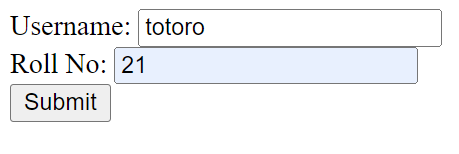
\includegraphics[width=8cm]{3/out.png}
  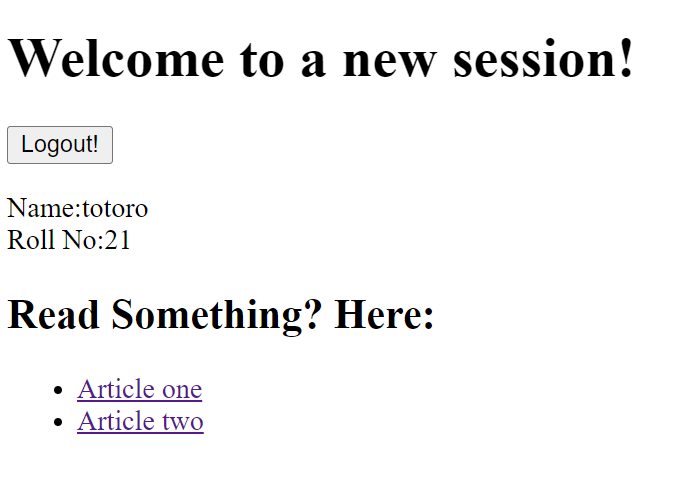
\includegraphics[width=10cm]{3/out2.png}
  
\includegraphics[width=10cm]{3/out3.png}
  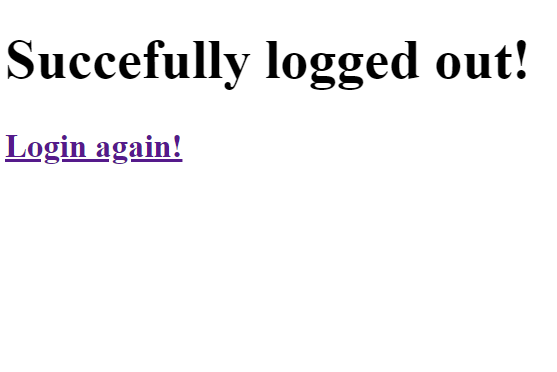
\includegraphics[width=10cm]{3/out4.png}
\end{figure}

\newpage
\section*{Question 4}
Write PHP code to retrieve record from the database and print it
in tabular form.

Consider following table:

\begin{tabular}{ | c | c | c |  c | c | }
  \hline
  Fields:   & Name    & Code & Designation & Salary \\
  Data Type & varchar & int  & varchar     & int    \\
  \hline
\end{tabular}

\subsection*{Code}
\lstinputlisting[language=php]{4/index.php}
\subsection*{Output}
\begin{figure}[H]
  \centering
  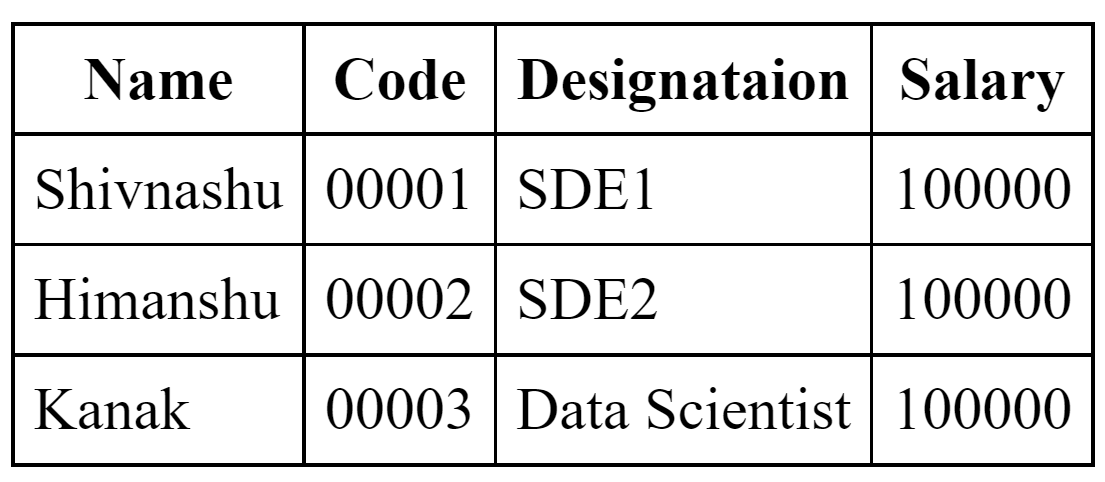
\includegraphics[width=10cm]{4/out.png}
\end{figure}

\newpage
\section*{Question 5}
Write PHP code to crete a form with following input, Name, Code, Designation and Salary.
Submit the form data into and insert these values in the database.

\subsection*{Code}
\textbf{index.php}
\lstinputlisting[language=php]{5/index.php}
\textbf{insert.php}
\lstinputlisting[language=php]{5/insert.php}
\newpage
\subsection*{Output}
\begin{figure}[H]
  \centering
  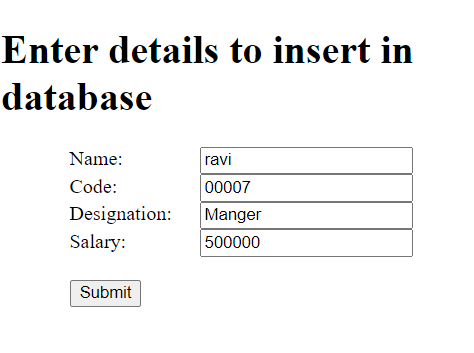
\includegraphics[width=10cm]{5/out.png}
  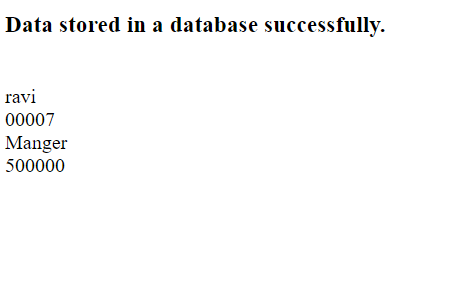
\includegraphics[width=10cm]{5/out2.png}
  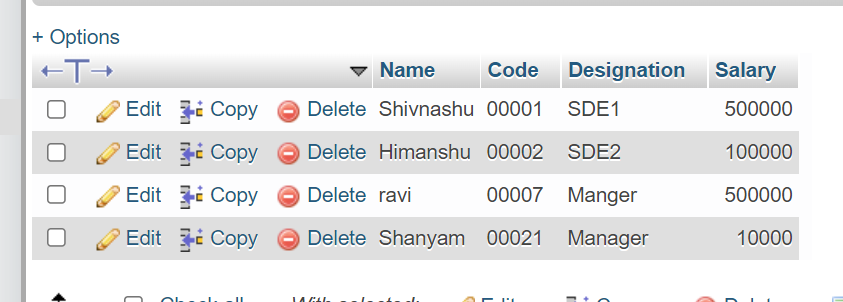
\includegraphics[width=14cm]{5/out3.png}
\end{figure}

\newpage
\section*{Question 6}
Write PHP code to update salary of an employer according to employee's code.
\subsection*{Code}
\textbf{insert.php}
\lstinputlisting[language=php]{6/index.php}
\textbf{update.php}
\lstinputlisting[language=php]{6/update.php}
\newpage
\subsection*{Output}
\begin{figure}[H]
  \centering
  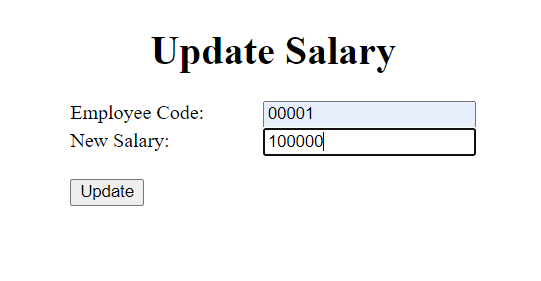
\includegraphics[width=10cm]{6/out.png}
  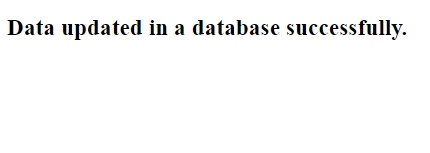
\includegraphics[width=10cm]{6/out2.png}
  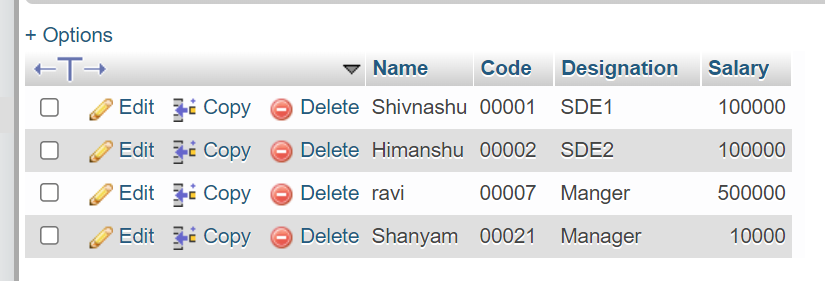
\includegraphics[width=14cm]{6/out3.png}
\end{figure}


\newpage
\section*{Question 7}
Write PHP code to delete particular employer record according to his employees code.
\subsection*{Code}
\textbf{index.php}
\lstinputlisting[language=php]{7/index.php}
\textbf{delte.php}
\lstinputlisting[language=php]{7/delete.php}
\newpage
\subsection*{Output}
\begin{figure}[H]
  \centering
  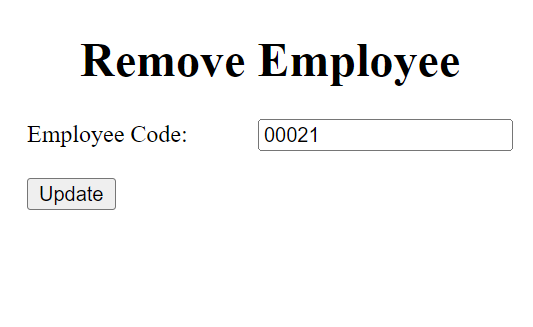
\includegraphics[width=10cm]{7/out.png}
  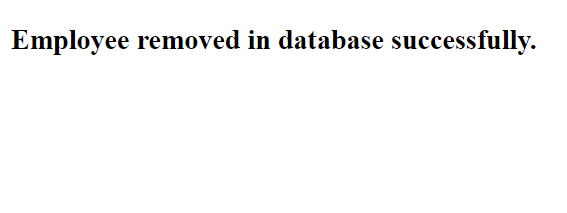
\includegraphics[width=10cm]{7/out2.png}
  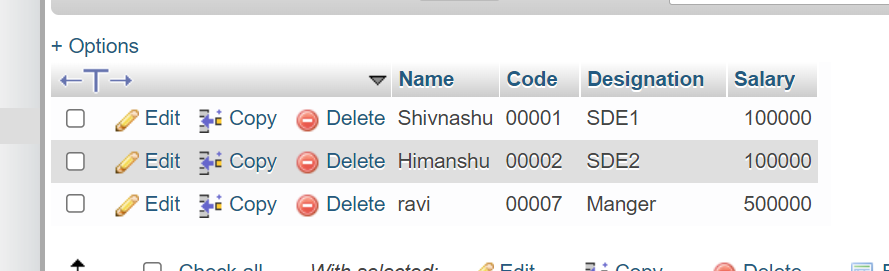
\includegraphics[width=14cm]{7/out3.png}
\end{figure}

\end{document}